\section{Validation and Results}
\label{sec:results}

\subsection{Regression Suites}

Every layer has a self-verifying suite
(Table~\ref{tab:suites}); all pass at the state documented here.

\begin{table}[H]
    \centering
    \caption{Verification suite summary.}
    \label{tab:suites}
    \small
    \begin{tabular}{@{}lrp{7.6cm}@{}}
    \toprule
    \textbf{Suite} & \textbf{Checks} & \textbf{Scope} \\
    \midrule
    \texttt{verify\_article.py} & 44 & bit-exact article worked examples:
        CRCs, Base38/QTH, conv-code outputs at all rates,
        scrambler/interleaver sequences, ZC ACF
        (Appendix~\ref{app:verify}) \\
    \texttt{smoke\_e2e.py}      & 10 & end-to-end TX$\to$channel$\to$RX
        incl.\ CFO, modes, STF, auto-mode detection \\
    \texttt{fixed\_point.py}    & 24 & fixed-point primitives, TX/RX
        parity, LDPC and 16-QAM TX and RX, HARQ, calibration, SNR
        estimator (Appendix~\ref{app:fixed}) \\
    \texttt{rf\_channel.py}     &  6 & SSB transparency, LO-derived CFO
        to 0.1\,Hz, decode through the fading RF chain \\
    \texttt{afc\_netting.py}    & --- & netting convergence +
        trim-budget and anchor guard scenarios (PASS/FAIL) \\
    \texttt{simplex\_session.py}& --- & whole-system two-station test,
        bit-exact delivery assert (PASS/FAIL) \\
    \bottomrule
    \end{tabular}
\end{table}

\subsection{Article Reproduction}

\begin{table}[H]
    \centering
    \caption{Reproduction versus the article.}
    \label{tab:reproduction}
    \small
    \begin{tabular}{@{}lll@{}}
    \toprule
    \textbf{Metric} & \textbf{Article} & \textbf{This implementation} \\
    \midrule
    Worked examples & --- & 44/44 bit-exact \\
    Sensitivity, BPSK 1/3 & $\approx -7.5$\,dB &
        $-7.2$\,dB raw RX; $-7.6$\,dB genie-synchronized \\
    BER/PER curves (Figs.~23--24) & simulated &
        reproduced (Figure~\ref{fig:berper}), both preambles \\
    \bottomrule
    \end{tabular}
\end{table}

The remaining 0.3\,dB between the raw and genie-synchronized receiver
is residual synchronization loss at low SNR (occasional missed
detections and one-symbol timing slips), not the decode chain ---
i.e.\ the reproduction gap is closed to within measurement noise of
its diagnosed cause.

\begin{figure}[H]
    \centering
    \begin{subfigure}{0.49\textwidth}
        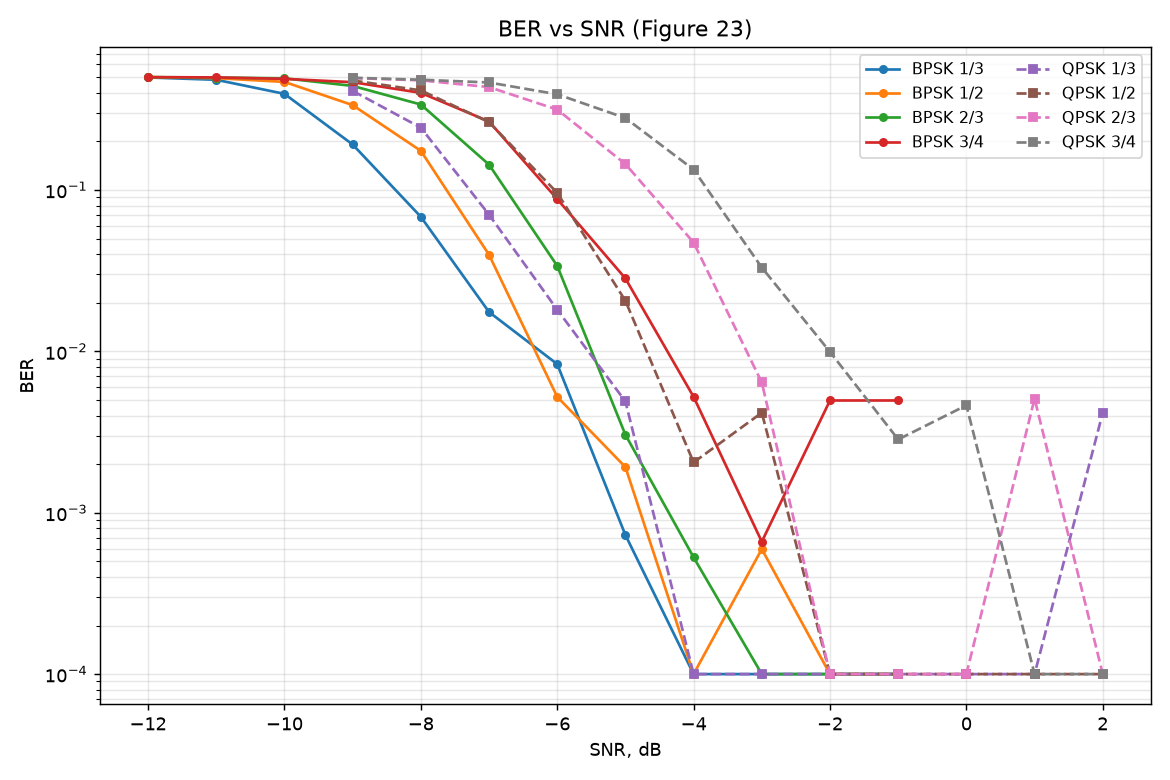
\includegraphics[width=\textwidth]{images/ber_vs_snr.png}
        \caption{BER versus SNR.}
    \end{subfigure}
    \hfill
    \begin{subfigure}{0.49\textwidth}
        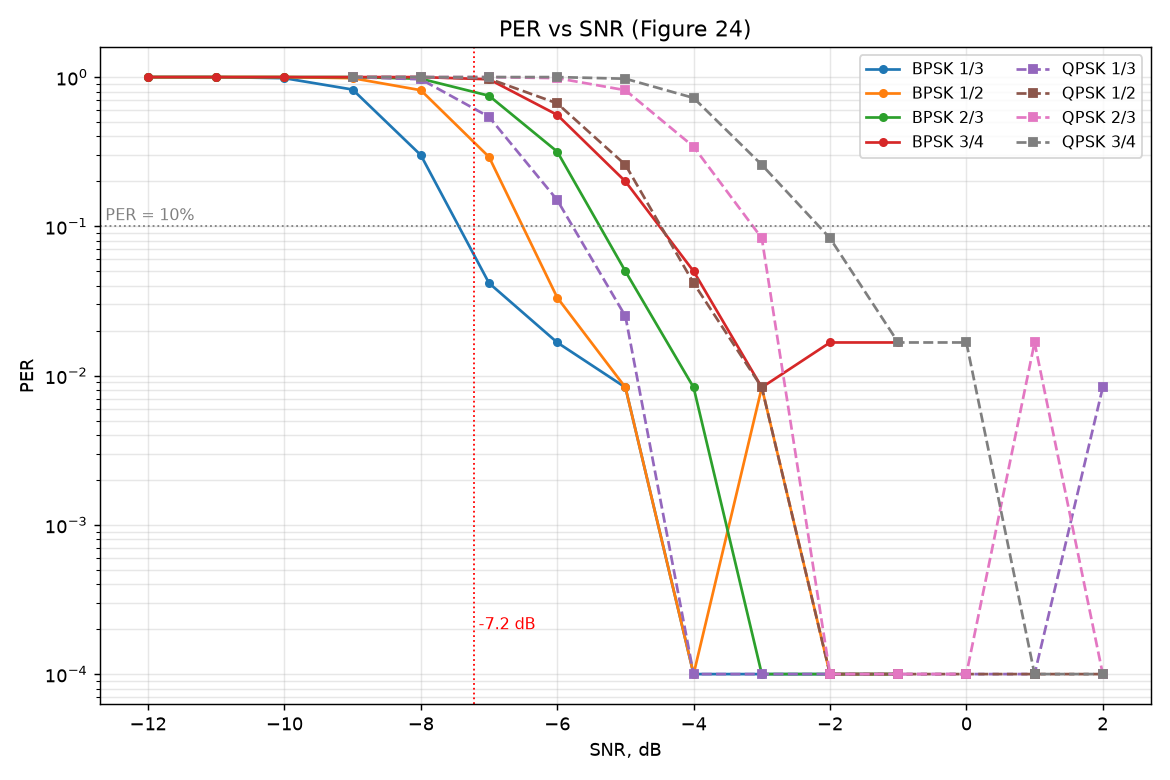
\includegraphics[width=\textwidth]{images/per_vs_snr.png}
        \caption{PER versus SNR.}
    \end{subfigure}
    \caption{Reproduction of the article's Figures~23--24: eight
             modulation/rate configurations over the article channel
             model (multipath $[1,0,0.4,0,0,0.2]$, BSC $10^{-3}$, BEC
             $2\cdot 10^{-2}$, random $\pm 100$\,Hz CFO with drift,
             random timing), 120 packets per point.}
    \label{fig:berper}
\end{figure}

\begin{figure}[H]
    \centering
    \begin{subfigure}{0.49\textwidth}
        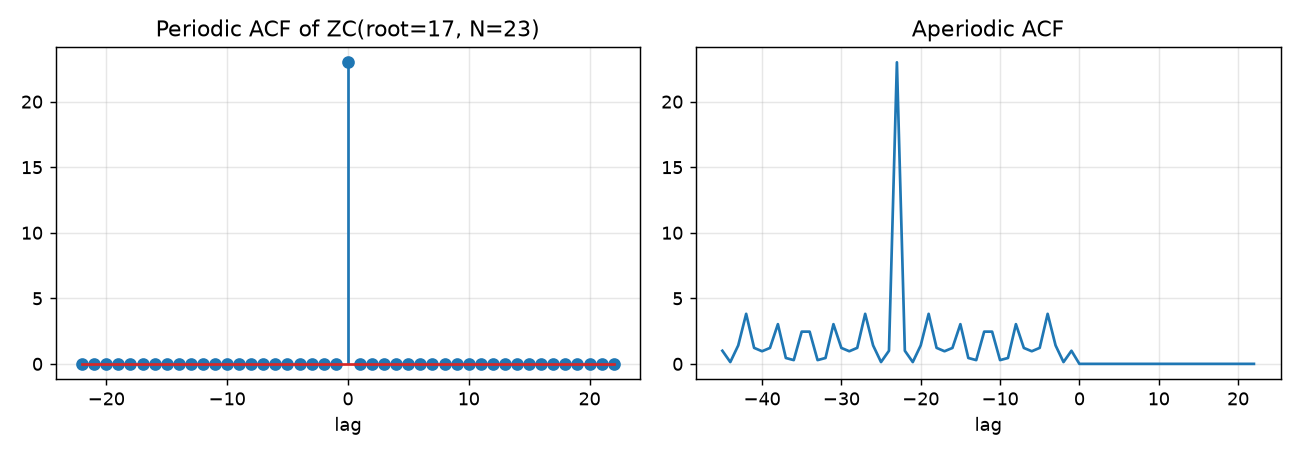
\includegraphics[width=\textwidth]{images/zc_acf.png}
        \caption{Zadoff--Chu autocorrelation.}
    \end{subfigure}
    \hfill
    \begin{subfigure}{0.49\textwidth}
        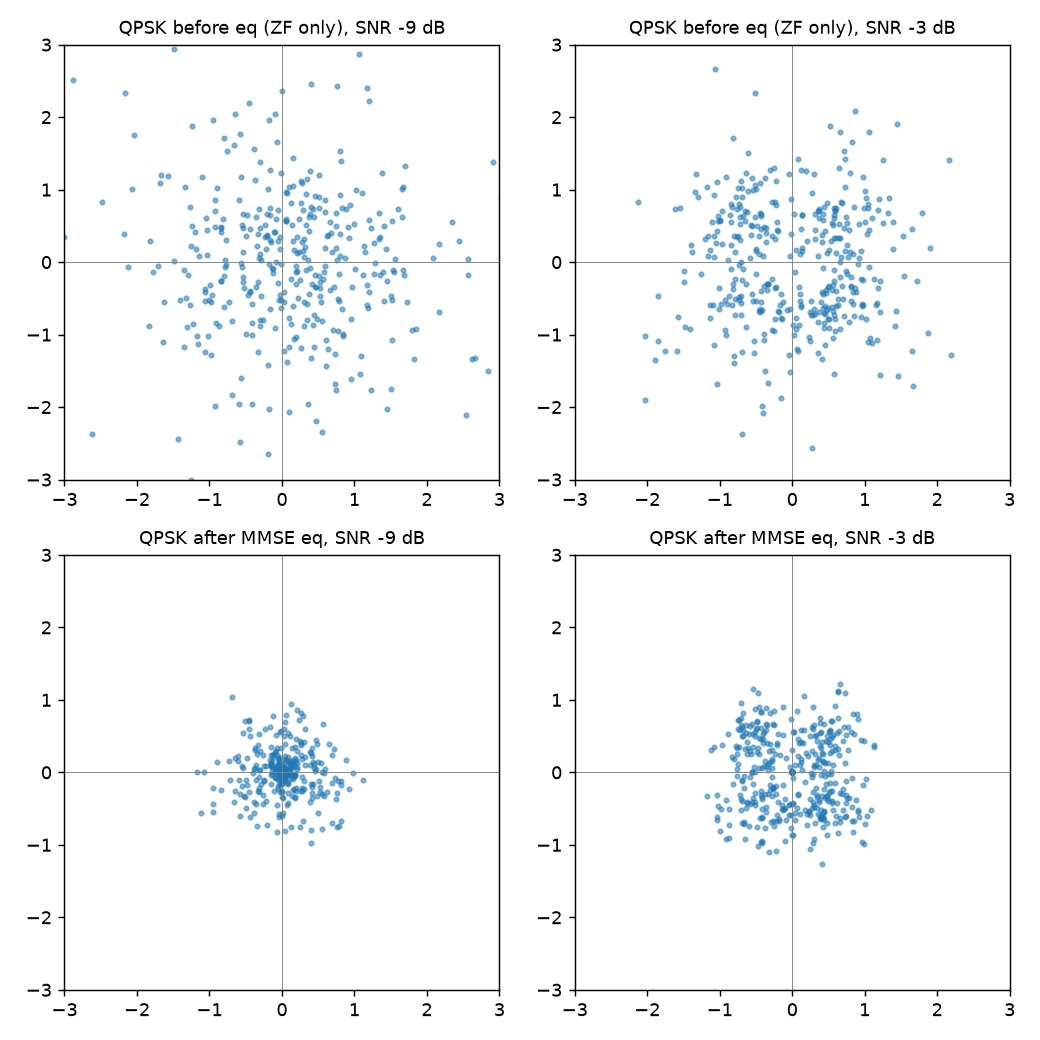
\includegraphics[width=\textwidth]{images/constellation_qpsk.png}
        \caption{QPSK constellation, before/after equalization.}
    \end{subfigure}
    \caption{Article-style diagnostic figures
             (\texttt{experiments/figures.py}).}
    \label{fig:diag}
\end{figure}

\subsection{Measured Feature Gains}

Table~\ref{tab:gains} consolidates every A/B-measured improvement.
All A/B comparisons use fixed seeds (same channel realizations per
arm); sensitivity points use 40--120 trials.

\begin{table}[H]
    \centering
    \caption{Feature gains, A/B measured.}
    \label{tab:gains}
    \small
    \begin{tabular}{@{}p{4.6cm}p{9.6cm}@{}}
    \toprule
    \textbf{Feature} & \textbf{Measured effect} \\
    \midrule
    LLR recalibration & $+1.5$--2\,dB on BPSK/QPSK rungs ($-9$\,dB:
        6/40 $\to$ 29/40); regresses 16-QAM $\to$ gated to
        $\mu \le 2$ \\
    HARQ chase combining & 2nd attempt 15/20 vs.\ 10/20 at
        $-8.5$\,dB (noise-limited regime) \\
    LDPC (IRA 768/256) vs.\ conv & $+0.7$\,dB AWGN at BLER 10\,\%;
        $\approx$ parity end-to-end (front-end LLR quality binds) \\
    STF preamble variant & equal to Newman everywhere ($\pm 0.14$\,dB
        over 8 configs, $2\sigma$ agreement per point) \\
    AFC netting & $+284$\,Hz $\to$ $<12$\,Hz in 5 exchanges; steady
        $\le 11$\,Hz under 0.09\,Hz/s relative drift \\
    Fixed-point RX vs.\ float & $\le 0.5$\,dB loss at $-7$\,dB;
        \emph{ahead} at $-9/-10$\,dB (22 vs.\ 20, 11 vs.\ 5 of 30,
        against float+recal); 16-QAM within 0.3--0.8\,dB after
        per-modulation LLR quantization (8-bit for $\mu = 4$) \\
    Integer SNR estimator & $\le$1.5\,dB error, $-17\ldots+8$\,dB, all
        modes; gain weighting essential (equal-weight pooling was
        5--15\,dB pessimistic on faded EXTREME frames) \\
    \bottomrule
    \end{tabular}
\end{table}

\subsection{The System Demonstration}

The recorded demonstration (\texttt{results/system\_demo.wav},
Figure~\ref{fig:timeline}, transcript in Appendix~\ref{app:demo}) is
the whole system at once: two stations over the fading SSB RF chain
with realistic LO errors, EXTREME-mode negotiation, rate climb,
AFC netting visible in the transcript's CFO column, HARQ, and
bidirectional message transfer --- blind-decoded from the monitor's
audio by \texttt{demod\_frame\_auto} with no side information.

\begin{figure}[H]
    \centering
    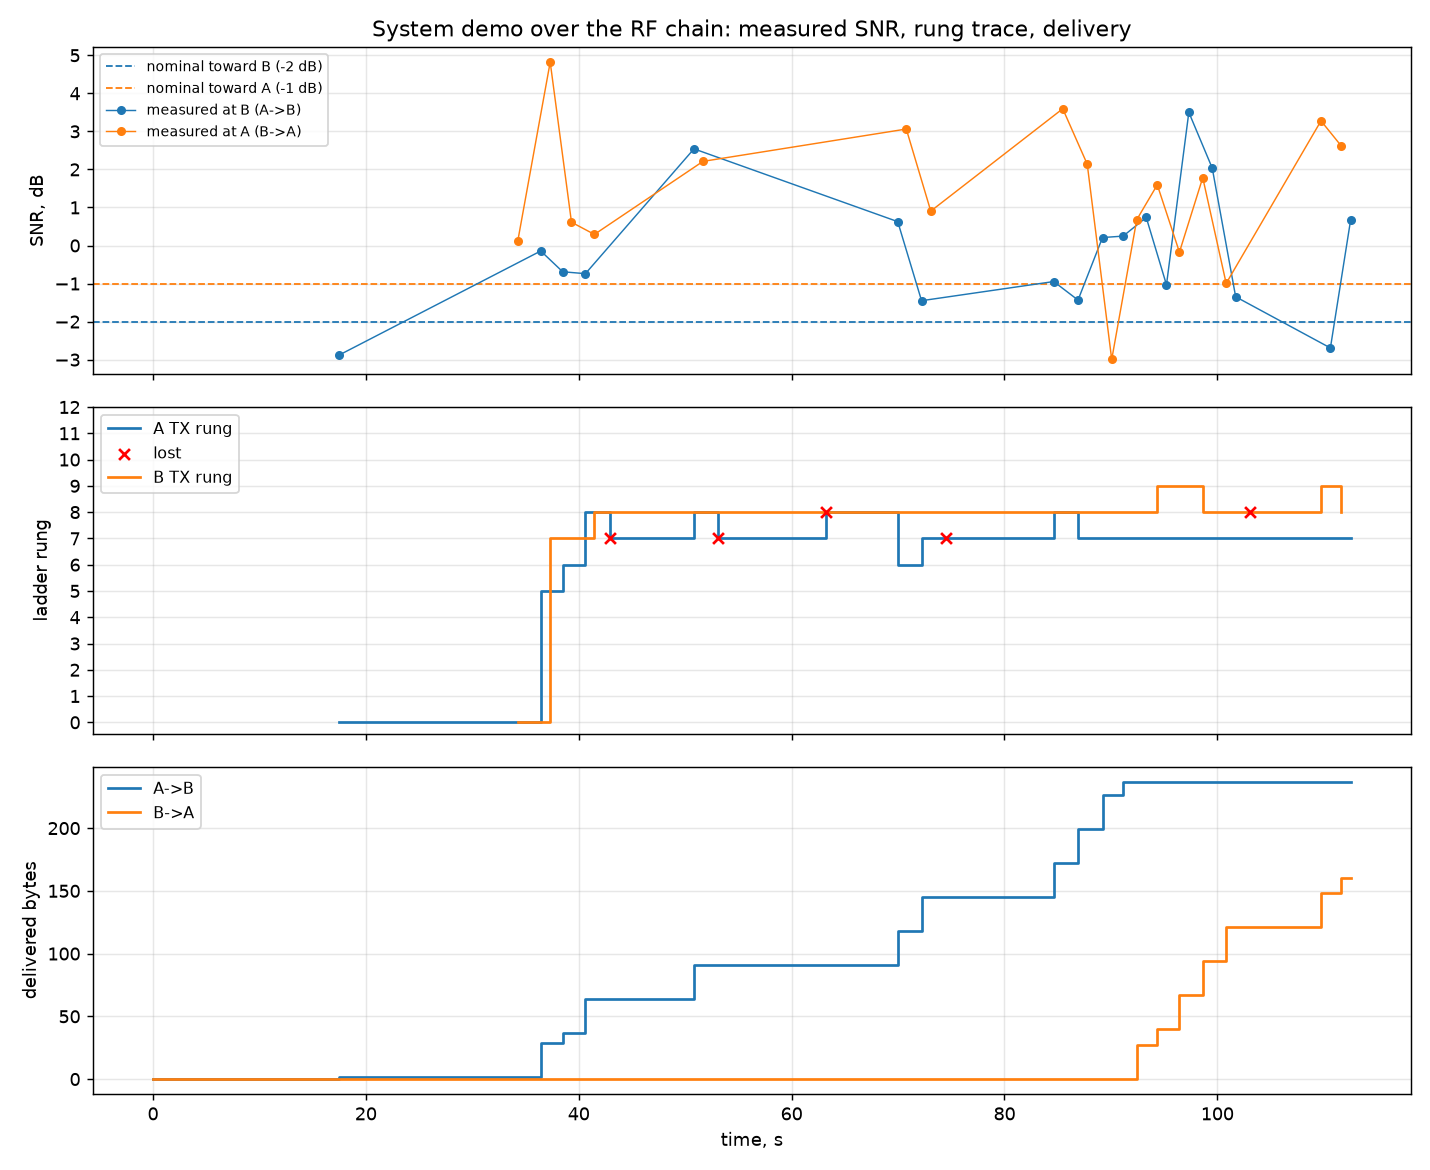
\includegraphics[width=\textwidth]{images/system_demo_timeline.png}
    \caption{System-demo timeline: per-frame SNR, ladder rungs, and
             delivery over the session.}
    \label{fig:timeline}
\end{figure}

The same demonstration also exists on the \emph{fixed-point} pipeline
(\texttt{-{}-phy fixed}, Section~\ref{sec:fixed}): at $-2/-1$\,dB
(\texttt{system\_demo\_fixed.wav}, 37/47 frames blind-decoded) and at
$+5$\,dB, where the ladder climbs into 16-QAM
(\texttt{system\_demo\_fixed\_qam16.wav}, 26/40;
Figure~\ref{fig:fixed_timeline} and Appendix~\ref{app:fixeddemo}).

\begin{figure}[H]
    \centering
    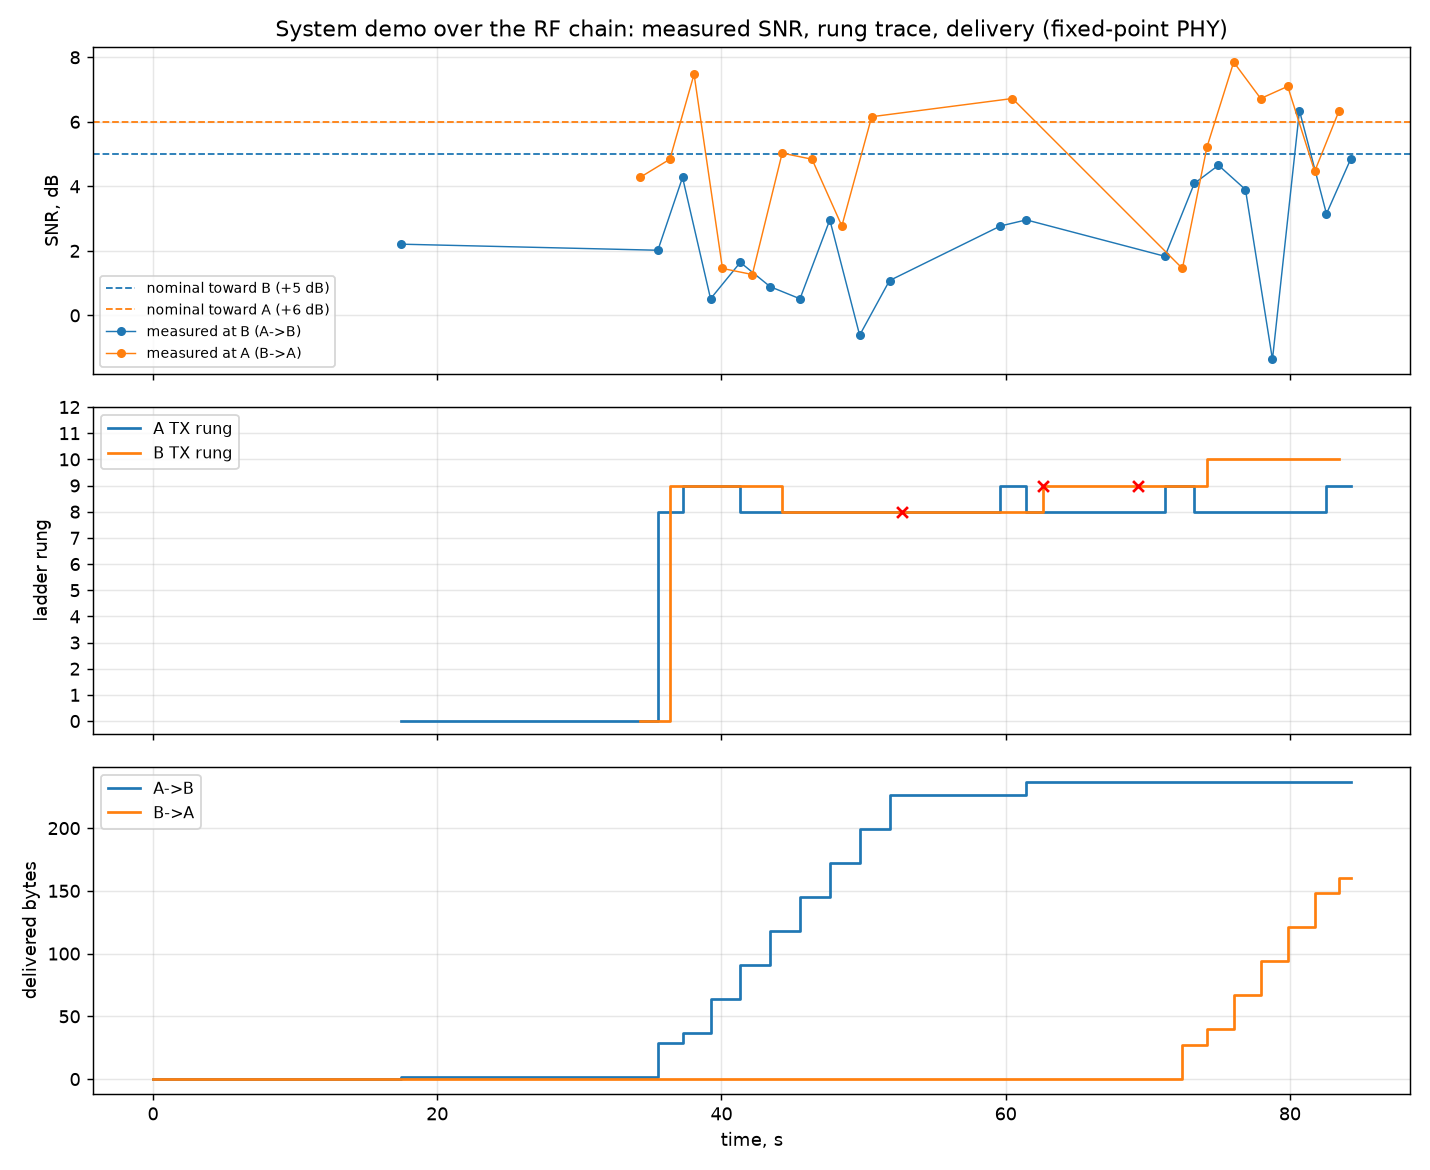
\includegraphics[width=\textwidth]{images/system_demo_fixed_qam16_timeline.png}
    \caption{Fixed-point-pipeline demo at $+5$\,dB: the integer SNR
             estimates drive the ladder into the 16-QAM rungs.}
    \label{fig:fixed_timeline}
\end{figure}

\subsection{Link Budget}

In radio terms, the EXTREME operating point ($-17.5$\,dB planned,
$-17.9$\,dB measured, 6\,kHz reference) needs
$S/N_0 \approx +20.3$\,dB-Hz, i.e.\ $\approx -13.7$\,dB in the
ham-standard 2.5\,kHz bandwidth --- about 7\,dB less sensitive than
FT8~\cite{ft8} and $\sim$20\,dB better than SSB voice.  Against
ITU-R~P.372 noise levels~\cite{itu_p372} with 0\,dBi antennas: on
80\,m at 10\,W, 500--2000\,km reliably on typical nights and
3000--5000\,km from quiet rural sites; on 40\,m at 10\,W,
300--1500\,km all day and worldwide multi-hop on quiet winter nights;
100\,W adds roughly one ionospheric hop to everything.  A planning
caveat: EXTREME's 0.69\,s coherent integration assumes
$\lesssim$0.1\,Hz Doppler spread --- on disturbed or auroral paths
($\ge$1\,Hz) the coherent gain collapses at any power and ROBUST is
the better choice, one more argument for adaptive mode selection.

\subsubsection{Measured Against a Reference Source}
\label{sec:link_budget_measured}

Everything above is derived from a \emph{relative} sensitivity and an
\emph{assumed} noise figure.  With the SDR receiver of
Section~\ref{sec:cport_sdr} on the bench, the assumption can be
replaced by a measurement: a tinySA's calibration output, a reference
tone at a documented level, was fed into the radio through a 40\,dB
attenuator and the receive chain characterised end to end
(\texttt{demoapp/sdr\_rx\_calibrate.py};
\texttt{results/sdr\_rx\_calibration.csv}).  At 10\,MHz with
$-65$\,dBm at the antenna port:

\begin{table}[H]
    \centering
    \caption{Receive chain measured against a reference source
             (HackRF One, LNA 40\,dB).}
    \label{tab:rx_calibration}
    \small
    \begin{tabular}{@{}lp{8.2cm}@{}}
    \toprule
    \textbf{Quantity} & \textbf{Measured} \\
    \midrule
    Frequency error & $-33.1$\,Hz at 10\,MHz $= -3.31$\,ppm, repeatable
                      to 0.0\,Hz ($-23$\,Hz at 7\,MHz) \\
    Linearity       & 1.002\,dB/dB over 16\,dB of gain, 0.03\,dB
                      residual \\
    Receiver noise  & $-95.5$\,dBm in the 6\,kHz reference band
                      (NF $\approx$ 40\,dB) \\
    \midrule
    \multicolumn{2}{@{}l}{\textit{Absolute sensitivity} $=$ measured
      noise floor $+$ the rung's required SNR:} \\
    rung 0 \; EXTREME BPSK 1/3 \; 7.8\,bit/s   & $-113.4$\,dBm \\
    rung 4 \; NORMAL BPSK 1/3 \; 117.6\,bit/s  & $-103.1$\,dBm \\
    rung 12 \; NORMAL 16-QAM 3/4 \; 1059\,bit/s & $-90.8$\,dBm \\
    \bottomrule
    \end{tabular}
\end{table}

Two results matter for planning.  First, the receiver's own noise is
\emph{not} what limits this link: against ITU-R~P.372 atmospheric noise
in the same 6\,kHz band, external noise still dominates by $+9$\,dB at
a quiet rural site, $+17$\,dB at a typical rural one and $+24$\,dB in
residential noise --- so the externally-limited assumption behind the
ranges above holds, and it holds with about 9\,dB of margin at the
quietest sites.  That margin is precisely where a preselector and a
low-noise amplifier begin to pay for themselves, and it is worth noting
that the 40\,dB noise figure measured here belongs to a wideband,
8-bit, unpreselected SDR --- an ordinary HF receiver is far better, so
this is close to a worst case.

Second, the frequency error is negligible for this waveform: 3.31\,ppm
against an acquisition range that tolerates roughly 50\,ppm at 7\,MHz.
A free-running SDR needs no external reference to \emph{acquire} a
frame; a disciplined oscillator matters only for EXTREME's 0.69\,s
coherent integration, where drift \emph{within} a 44\,s frame is the
constraint rather than absolute accuracy.  The absolute levels in
Table~\ref{tab:rx_calibration} inherit the calibration output's nominal
$-25$\,dBm; the relative results --- linearity, frequency error, and
the comparison against atmospheric noise --- do not.
